\appendix




\chapter{Covariance of the estimate}
\label{chp:MAP_covariance}
An important question to ask is how confident are we in our MAP estimate.
This can inform us on the quality of the performed estimation. In particular, in the case of parameter identification, a certain degree of excitation,
namely variability in the data, is necessary to obtain reliable values. Unfortunately, as we will see, the computation of the covariance on the posterior
is a costly process that is, therefore, rarely used in online estimation.

First we will review the process to obtain the posterior's covariance, known as the Laplacian approximation. Then we will give a simple example to
illustrate the nature of the approximation and compare it to an exact inference of the posterior distribution.

\section{Laplace approximation}
\label{sec:map_covariance}
Even if our priors and measurements models are Gaussian distributions, the posterior distribution
is in general non-Gaussian (unless all measurements models are linear). The region near the peak of the posterior is, however, often nearly Gaussian in shape.
The curvature around the mode is described by the Hessian of the posterior negative log-likelihood at the MAP estimated state. 
It can be shown that he Hessian is the \textit{information matrix} of the problem\footnote{The proof of this statement is out of the scope of this document and can be found in Section 5.1 of
\cite{peng2018advanced}}. Thus, finding the covariance of the MAP estimate resolves to inverting a 
sparse positive definite matrix.

\begin{equation}
    p(\cX | \cZ) \approx \Gaussian{\cX^{MAP}}{\bfH^{-1}}
    \label{eq:map_laplace}
\end{equation}

This is referred to as the quadratic or Laplace approximation (\cite{mcelreath2018statistical}, section 2.4.2). Obtaining an approximation of the full posterior is then a two-step process: 
first, find the mode of the posterior (the MAP), then "fit a Gaussian" on this mode. 

The full covariance is however rarely computed for a few reasons. First, few algorithms rely on this information (a notable exception being active feature matching \cite{davison2007monoslam}, which is not longer used in state of the art vision systems). Second, computing the Hessian's inverse is too costly to be realized "in the loop". Sometimes, only parts of the covariance are computed using the Schur-complement method \cite{konolige2005slam}, which is costly but much less than the full inverse.
The covariance computation is then often left for offline evaluations of the estimation.

To contrast this approach with the aforementioned approximations, variational inference as applied in Barfoot et al. 
\cite{barfoot2020exactly} for instance fit both the mean and the information matrix of a Gaussian model as a result of a single optimization problem.



\section{Example: stereoscopic depth estimation}

We can illustrate the Laplace approximation with a one-dimensional toy problem (borrowed from Barfoot \cite{barfoot2017state}, section 4.1.1).
The problem is stated as estimating the depth $x \in \Reals$ of a landmark in the scene with a nonlinear camera model (see \figRef{fig:barfoot_stereo})
%
\begin{equation}
    y = \frac{fb}{x} + n_y
\end{equation}
%
%
\begin{figure}[h]
    \centering
    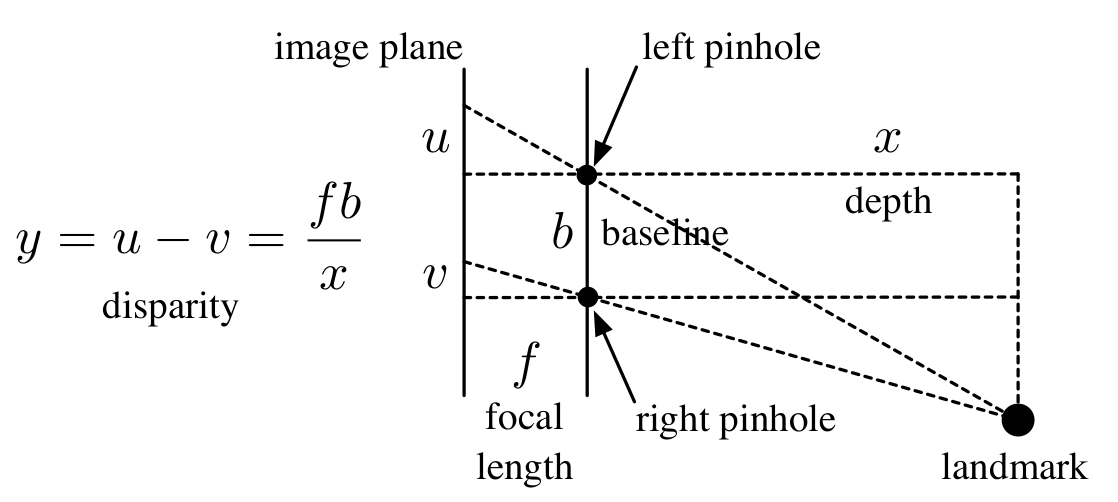
\includegraphics[width=0.6\textwidth]{figures/barfoot_stereo.png}
    \caption{Stereo depth estimation toy model \cite{barfoot2017state}}
    \label{fig:barfoot_stereo}
 \end{figure}
%
where $y=u - v$ is a disparity measurement ($u$ and $v$ are pixels corresponding to the projection of the landmark in each camera), $f$ is the focal
length of the cameras (in pixels), $b$ is the horizontal distance between cameras (the baseline, in meters), and $n_y \approx \Gaussian{0}{\sigma_y^2}$ 
is the measurements noise (in pixels), assumed to be Gaussian. We also assume that we have prior knowledge about the 
estimated value $x_p$, with a standard deviation of $\sigma_p$.

To ground the problem, we will assign sensible values to the problem (same as \cite{barfoot2017state}):
%
\begin{gather*}
    x_{true} = 22~[m], \quad x_p = 20~[m], \quad \sigma_p = 3~[m] \\
    f = 400~[pixels], \quad b = 0.1~[m], \quad \sigma_y = 0.3~[pixels]   
\end{gather*}
%
where $x_{true}$ is the true depth that we seek to estimate.

Notice that the prior standard deviation is quite big, assuming a great uncertainty about the prior value. We simulate noisy measurements by drawing samples 
$\{y_{i \in [1..m]}\}$ of the measurement model using $x_{true}$ (we drew $m=10$ measurements). For a low dimensional problem such as this one, 
it is possible to compute the full posterior distribution $p(x|\bfy)$ by numerical integration, which is referred to as the "grid approximation" by 
\cite{mcelreath2018statistical}. We can make this computation almost arbitrarily precise since the computations are quite cheap. The prior and density distribution are represented in \figRef{fig:MAP_stereo1D}. Applying the Laplacian approximation to
compute a posterior approximation involves minimizing the negative log-likelihood:

\begin{equation}
    \frac{1}{2 \sigma_p^2}(x - x_p)^2 + \frac{1}{2\sigma_y^2} \sum_{i=1}^m (\frac{fb}{x} - y_i)
\end{equation}

Finding the MAP and approximating the covariance deviation of $x$, we can plot the MAP posterior along with its numerical computation in \figRef{fig:MAP_stereo1D}. 
Both computations result in largely overlapping functions: the main mass of the real posterior density function is captured by the Laplacian approximation.
However, notice that the real posterior distribution is not symmetrical contrary to the prior it derives from. This means that, contrary to its Gaussian approximation, the mean of the
of the real posterior is not equal to its mode. 

\begin{figure}[h]
    \centering
    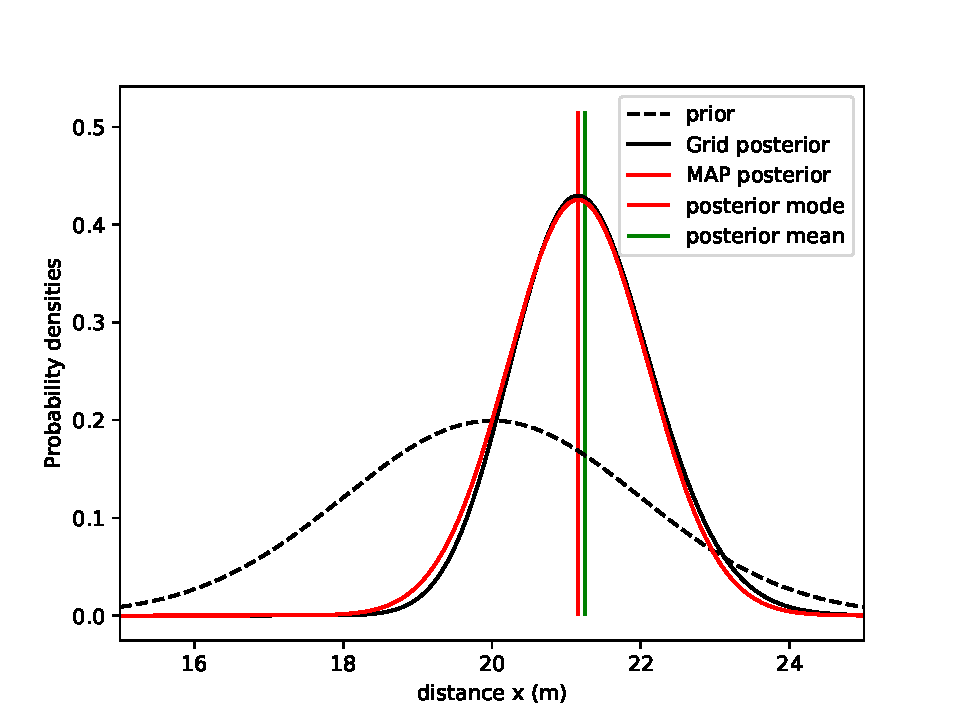
\includegraphics[width=0.8\textwidth]{figures/MAP_stereo1D.pdf}
    \caption{Representation of the posterior distribution inference for the 1D depth estimation problem. Dotted black: prior on $x$, 
    continuous black: numerical "grid" integration of the posterior, continuous red: Laplacian approximation of the posterior. 
    Vertical lines: red=MAP, green=mean of the posterior. The true value (22 m) is reasonably close to the MAP given the variance 
    of the posterior distribution.
    }
    \label{fig:MAP_stereo1D}
 \end{figure}







\chapter{Pre-integration details}
\section{Justification of \cite{forster2017-TRO} delta formulas}
\label{sec:forster_proof}
We detail here how the delta formulas of equation \eqRef{eq:IMUPreintij} can be derived from \eqRef{eq:IMUIntim}.

The rotation one is easy to get, multiplying by $\Rot{}{}^{i,T}$:
\begin{equation}
    \DR_{im} \triangleq \Rot{}{}^{i,T} \Rot{}{}^{m} = \prod_{k=i}^{m} \Exp((\angvelm{}{}^k - \bias_{\angvel{}{}}^k - \noise_{\angvel{}{}}^k)\dt)
    \label{eq:IMUDeltaR}
\end{equation}

The velocity is as well quite easy, by defining $\Dt_{im} \triangleq \sum_{k=i}^{m} \dt = (m-i)\dt$:
\begin{equation}
    \Dv_{im} \triangleq \Rot{}{}^{i,T} (\vel{}{m} - \vel{}{i} - g \Dt_{im}) 
    = \prod_{k=i}^{m} \DR_{ik} \Exp((\accm{}{}^k - \bias_{\acc{}{}}^k - \noise_{\acc{}{}}^k)\dt)
    \label{eq:IMUDeltav}
\end{equation}

The position delta requires more calculations. First, inject equation \eqRef{eq:IMUDeltav} in the position equation of \eqRef{eq:IMUIntim} then rearrange and reorder the terms.

\begin{equation}
\begin{split}
\posi{}{}^{m} - \posi{}{}^{i} &= \sum_{k=i}^{m} \Big[
(\vel{}{}^i + \grav \Dt_{ik} + \Rot{}{}^i \Dv_{ik})\dt 
+ \frac{1}{2}\grav \dt^2 + \frac{1}{2}\Rot{}{}^{k}(\accm{}{}^k - \bias_{\acc{}{}}^k - \noise_{\acc{}{}}^k)\dt^2 \Big]
\\
&= \vel{}{}^i \Dt_{im} + 
\grav\sum_{k=i}^{m} \Dt_{ik} \dt + \frac{1}{2}\grav \sum_{k=i}^{m} \dt^2 +
\Rot{}{}^i\sum_{k=i}^{m} \Big[\Dv_{ik}\dt +  \frac{1}{2} \DR_{ik} (\accm{}{}^k - \bias_{\acc{}{}}^k - \noise_{\acc{}{}}^k)\dt^2 \Big]
\\
&= \vel{}{}^i \Dt_{im} + 
\grav \sum_{k=i}^{m} (\Dt_{ik} \dt + \frac{1}{2}\dt^2) +
\Rot{}{}^i\sum_{k=i}^{m} \Big[\Dv_{ik}\dt +  \frac{1}{2} \DR_{ik} (\accm{}{}^k - \bias_{\acc{}{}}^k - \noise_{\acc{}{}}^k)\dt^2 \Big]
\end{split}
\end{equation}

We will simplify the gravity term that we will call $\cG t_{im}$. Noting that:

\begin{equation*}
    \sum_{k=i}^{m}k = \sum_{k=1}^{m}k - \sum_{k=1}^{i-1}k = \frac{m(m-1)}{2} - \frac{i(i-1)}{2} 
\end{equation*}

we can deduce that:

\begin{equation*}
\begin{split}
\cG t_{im} 
&= \dt \sum_{k=i}^{m}(\Dt_{ik} + \frac{1}{2}\dt) = \dt \sum_{k=i}^{m}((k -i)\dt + \frac{1}{2}\dt)
\\
&= \dt \Big[ \sum_{k=i}^{m} [ k \dt - i(m-i)\dt ] + \frac{1}{2}\Dt_{im}  \Big] 
\\
&= \dt \Big[ \frac{\dt}{2} (m(m-1) - i(i-1) - 2i(m-1)) + \frac{1}{2}\Dt_{im} \Big] 
\\
&= \dt \Big[ \frac{\dt}{2} (i^2 - 2im + m^2 + i - m) + \frac{1}{2}\Dt_{im} \Big] 
\\
&= \dt \Big[ \frac{1}{2} (m-i)^2dt - \frac{1}{2}(m - i)\dt + \frac{1}{2}\Dt_{im} \Big]
\\
&= \frac{1}{2} (m-i)^2dt^2 = \frac{1}{2} \Dt_{im}^2
\end{split}
\end{equation*}
Multiplying by $\Rot{}{}^{i,T}$ and reordering the terms, we can finally define a position delta quantity:

\begin{equation}
    \Dp_{im} \triangleq \Rot{}{}^{i,T}(\posi{}{}^m - \posi{}{}^i - \vel{}{}^i \Dt_{im} - \frac{1}{2} \grav \Dt_{im}^2) = 
    \sum_{k=i}^{m} \Big[\Dv_{ik}\dt +  \frac{1}{2} \DR_{ik} (\accm{}{}^k - \bias_{\acc{}{}}^k - \noise_{\acc{}{}}^k)\dt^2 \Big]
\end{equation}


\section{Elements of the IMU delta matrix Lie group}
\label{sec:IMULieGroup}

\subsection{Tangent space and Lie algebra \texorpdfstring{$\mathfrak{d}$}{d}}
\cite{sola2018micro}
Following \cite{sola2018micro}, the tangent space of $\cD$ at the point $\D$ is found by taking the time derivative of the group constraint, $\D\inv\D = \bfI$.
Noting $\dot{\bullet} \te \dpar{\bullet}{t}$, this yields 
% the tangent space constraint, $\D\inv\dot\D+\dot{(\D\inv)}\D=0$.
% This gives 
after a few manipulations
%
\begin{align}\label{equ:constr}
\D\inv\dot\D 
&=
\begin{bsmallmatrix}
\hatx{\bw} & ~~\DR\tr\bfa~~ & \DR\tr(\bfv-\Dv) \\
\bf0 & 0 & 1 \\
\bf0 & 0 & 0 
\end{bsmallmatrix}
~,
\end{align}
%
with $\bfv \te \dot\Dp$, $\bfa \te \dot\Dv$ and $\hatx{\bw} \te \DR\tr\dot\DR$.
% The equation above defines the tangent space at the point $\D$. 
The Lie algebra $\mathfrak{d}$ is the tangent space at the identity $\D=\bfI$.
Its elements $\bm\nu\hhat 
\te \dot\D |_{\D=\bfI}$ and their isomorphics $\bm\nu$ in Cartesian space are given by, % $\D=\bfI$, so
%
\begin{align}
\bm\nu\hhat 
% \te \dot\D |_{\D=\bfI}
&=
\begin{bsmallmatrix}
\hatx{\bw} & \bfa & \bfv \\
\bf0 & 0 & 1 \\
\bf0 & 0 & 0 
\end{bsmallmatrix} \in \mathfrak{d}
~~~\xrightleftharpoons[\wedge]{~\vee~}~~~ 
\bm\nu=\begin{bsmallmatrix}
\bfv \\ \bfa \\ \bw \\ 1
\end{bsmallmatrix} \in\bbR^{10}
~.
\end{align}
%
This tangent $\bm\nu\hhat$ corresponds to the `velocity' of the group element. 
Any point in the Lie algebra can be obtained after moving at constant velocity during a period $\Dt$, that is, $\bftau\hhat=\bm\nu\hhat\Dt\in\mathfrak{d}$ ---see \eqRef{equ:lie_algebra}.
%
\subsection{The exponential map}
\subsubsection{The general case}
Eq.~\eqRef{equ:constr} can be written as $\dot\D=\D\cdot\bm\nu\hhat$.
This is an ordinary differential equation whose  integral for constant $\bm\nu$ yields the exponential map \cite{sola2018micro}, $ \D(t) = \exp\left(\bm\nu\hhat t\right)$.
This gives a direct expression of the integral of information of the type $(\bfv,\bfa,\bw)$ onto the deltas manifold. See below for the $(\bfa,\bw)$ case.
The closed form of the exponential map is obtained through Taylor expansion (see \eg\ \cite{sola2018micro}\ for examples). 
At $t=\Dt$ we have,
%
\begin{align}
\D(\Dt) 
&= \exp(\bm\nu\hhat\Dt) \te \sum_n \frac1{n!}(\bm\nu\hhat\Dt)^n
~.
\end{align}
%
% with $\bfA=\bftau\hhat\Dt$.
%
Exploiting the cyclic pattern of the powers of $\hatx{\bw}$, this results in
%
\begin{align}
\exp\left(\begin{bsmallmatrix}
\hatx{\bw} & \bfa & \bfv \\
\bf0 & 0 & 1 \\
\bf0 & 0 & 0 
\end{bsmallmatrix}\Dt\right) 
\!=\! \begin{bsmallmatrix}
\exp(\hatx{\bw}\Dt) & \bfQ\bfa\Dt\, & \bfQ\bfv\Dt+\bfP\bfa\Dt^2 \\
\bf0 & 1 & \Dt \\
\bf0 & 0 & 1
\end{bsmallmatrix}
\end{align}
%
with (we skip proofs for space reasons)
%
\begin{align} \label{equ:RQP}
% \bfR (\bth)
%  &= \exp(\hatx{\bth})
%   = \bfI + \sin\theta\hatx{\bfu} + (1-\cos\theta)\hatx{\bfu}^2\\
\bfQ (\bth)
 &= 
  \bfI + \frac{1-\cos\theta}{\theta}\hatx{\bfu} + \frac{\theta-\sin\theta}{\theta}\hatx{\bfu}^2\\
\bfP (\bth)
 &= 
  \frac12\bfI 
   + \frac{\theta-\sin\theta}{\theta^2}\hatx{\bfu} 
   + \frac{\cos\theta + \frac12\theta^2 - 1}{\theta^2}\hatx{\bfu}^2
~,
\end{align}
%
where  $\bth=\bw\Dt$, $\theta=\norm{\bth}$ and $\bfu=\bth/\theta$ form the angle-axis representation of the rotation step $\bw\Dt$. 


\subsubsection{The IMU case of \texorpdfstring{$\bfv=0$}{bfv=0}}
\label{sec:IMU_case}

We defined the IMU deltas as the motion relative to the free-falling frame, which has initial velocity $\bfv_i$. 
Thus the tangent velocity $\bfv=\dot\Dp$  is zero at the start of the integration step. 
%
Since the exponential $\Exp(\bm\nu\Dt)$ assumes a constant tangent vector $\bm\nu=(\bfv,\bfa,\bw,1)$ during the interval $\Dt$, we have that $\bfv=0$ during the full step. 
%
This gives immediately
%
\begin{align}
% \D &= 
\exp\left(\begin{bsmallmatrix}
\hatx{\bw} & \bfa & \bf0 \\
\bf0 & 0 & 1 \\
\bf0 & 0 & 0 
\end{bsmallmatrix}\Dt\right) 
= \begin{bsmallmatrix}
\exp(\hatx{\bw}\Dt) & ~\bfQ\bfa\Dt~ & \bfP\bfa\Dt^2 \\
\bf0 & 1 & \Dt \\
\bf0 & 0 & 1
\end{bsmallmatrix}
~.
\end{align}




\subsection{The adjoint and small adjoint matrices}

%
Following the general methodology explained in \cite{sola2018micro}, the adjoint matrix is obtained by identifying the linear terms in $\Ad{\D}\bftau=(\D\bftau\hhat\D\inv)\vvee$. We get after long but relatively easy calculations,
%
\begin{align}\label{equ:Ad}
\Ad{\D} &=
\begin{bsmallmatrix}
\DR & -\DR\Dt & \hatx{\Dp-\Dv\Dt}\DR & \Dv \\
\bf0 & \DR & \hatx{\Dv}\DR & \bf0 \\
\bf0 & \bf0 & \DR & \bf0 \\
\bf0 & \bf0 & \bf0 & 1
\end{bsmallmatrix} 
\quad
\in\bbR^{10\times10}~.
\end{align}



Similarly, from \cite{EADE-18-DERIVATIVE} the small adjoint matrix can be computed by identifying the linear terms in $
\ad{\bftau}\bfsigma = 
(\bftau\hhat\bfsigma\hhat-\bfsigma\hhat\bftau\hhat)^\vee
$
%
which  for $\bftau=(\bfrho,\bfupsilon,\bth,\Dt)\in\mathfrak{d}$ yields,
%
\begin{align}\label{equ:ad}
\mathrm{\bf ad}_\bftau = \begin{bsmallmatrix}
\hatx{\bth} & -\bfI\Dt & \hatx{\bfrho} & \bfupsilon \\
\bf0 & \hatx{\bth} & \hatx{\bfupsilon} & \bf0 \\
\bf0 & \bf0 & \hatx{\bth} & \bf0 \\
\bf0 & \bf0 & \bf0 & 0 
\end{bsmallmatrix}
\quad
\in\bbR^{10\times10}~.
\end{align}




\subsection{The right Jacobian}

The right Jacobian $\mjac{}{r}$ is the Jacobian of $\Exp()$ as described in \cite{sola2018micro}.
Lacking at the moment a closed form for it, we take the general methodology for the left Jacobian described in \cite{EADE-18-DERIVATIVE}, and transform it to the right using $\mjac{}{r}(\bftau)=\mjac{}{l}(-\bftau)$ \cite{sola2018micro},
%
\begin{align}\label{equ:Jr}
\mjac{}{r}(\bftau) 
= \mjac{}{l}(-\bftau) 
= \sum_i \frac{\ad{-\bftau}^i}{(i+1)!}
= \sum_i \frac{(-\ad{\bftau})^i}{(i+1)!}
% ~
% \in\bbR^{10\times10}
~.
\end{align}
%
This sum can be truncated at the desired degree of accuracy.






\section{Jacobians of force/torque pre-integration}

TODO

